\documentclass[11pt,a4paper]{article}
\usepackage[margin=2.2cm]{geometry}
\usepackage{amsmath,amssymb,bm}
\usepackage{booktabs}
\usepackage{tabularx}
\usepackage{xcolor}
\usepackage{hyperref}
\usepackage{tikz}
\usetikzlibrary{positioning,arrows.meta,calc}
\usepackage{enumitem}
\usepackage{float}
\usepackage[most]{tcolorbox}

\definecolor{hwblue}{RGB}{20,80,160}
\definecolor{resultbar}{RGB}{40,140,60}
\definecolor{resultbg}{RGB}{230,255,230}
\definecolor{warnbar}{RGB}{200,140,0}
\definecolor{warnbg}{RGB}{255,245,220}

\newtcolorbox{resultbox}[1][]{enhanced,breakable,
  colback=resultbg,colframe=resultbar,boxrule=0.6pt,
  left=4pt,right=4pt,top=4pt,bottom=4pt,
  title={\textcolor{resultbar}{\sffamily\bfseries Key Result} #1},
  attach boxed title to top left={yshift=-2mm,xshift=4mm},
  boxed title style={colback=resultbg,colframe=resultbar}}

\newtcolorbox{warnbox}[1][]{enhanced,breakable,
  colback=warnbg,colframe=warnbar,boxrule=0.6pt,
  left=4pt,right=4pt,top=4pt,bottom=4pt,
  title={\textcolor{warnbar}{\sffamily\bfseries Important} #1},
  attach boxed title to top left={yshift=-2mm,xshift=4mm},
  boxed title style={colback=warnbg,colframe=warnbar}}

\newcommand{\bq}{\bm{q}}
\newcommand{\bqd}{\dot{\bm{q}}}
\newcommand{\btau}{\bm{\tau}}
\newcommand{\bM}{\bm{M}}
\newcommand{\bC}{\bm{C}}
\newcommand{\bG}{\bm{g}}

\title{\textbf{Hardware-to-Simulation Methodology}\
\large Notes on CAD-Based Parameter Identification and Isaac Lab Actuator Calibration}
\author{Repo \texttt{exo-actuator-sensor-drivers}}
\date{May 2026}

\begin{document}
\maketitle

\begin{resultbox}
This note summarizes a practical sim-to-real methodology adapted from the
video transcript provided by the user.  The main idea is:
\begin{enumerate}[leftmargin=1.5em]
  \item build a physically credible URDF from measured hardware and CAD,
  \item tune the actuator model in Isaac Lab against real actuator data,
  \item only then train or evaluate policies for transfer to hardware.
\end{enumerate}
\end{resultbox}

\tableofcontents
\newpage

\section{Overview}

The methodology has three coupled parts:
\begin{enumerate}[leftmargin=2em]
  \item identify the rigid-body parameters used by the URDF,
  \item calibrate the simulated actuator model against real actuator response,
  \item close the remaining sim-to-real gap at the sensing and runtime level.
\end{enumerate}

\begin{figure}[H]
\centering
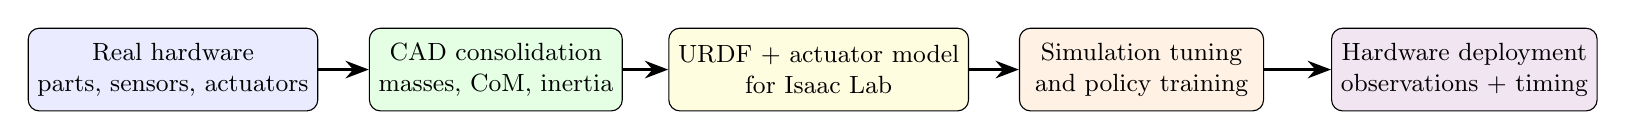
\begin{tikzpicture}[>=Stealth, every node/.style={font=\small, align=center}]
  \def\bw{3.1cm}
  \def\bh{1.05cm}

  \node[draw, rounded corners=4pt, fill=blue!8,
        minimum width=\bw, minimum height=\bh] (hw) at (0,0)
        {Real hardware\\parts, sensors, actuators};
  \node[draw, rounded corners=4pt, fill=green!10,
        minimum width=\bw, minimum height=\bh] (cad) at (4.1,0)
        {CAD consolidation\\masses, CoM, inertia};
  \node[draw, rounded corners=4pt, fill=yellow!12,
        minimum width=\bw, minimum height=\bh] (urdf) at (8.2,0)
        {URDF + actuator model\\for Isaac Lab};
  \node[draw, rounded corners=4pt, fill=orange!10,
        minimum width=\bw, minimum height=\bh] (sim) at (12.3,0)
        {Simulation tuning\\and policy training};
  \node[draw, rounded corners=4pt, fill=violet!10,
        minimum width=\bw, minimum height=\bh] (deploy) at (16.4,0)
        {Hardware deployment\\observations + timing};

  \draw[->, very thick] (hw) -- (cad);
  \draw[->, very thick] (cad) -- (urdf);
  \draw[->, very thick] (urdf) -- (sim);
  \draw[->, very thick] (sim) -- (deploy);
\end{tikzpicture}
\caption{Overall methodology: accurate rigid-body parameters and actuator calibration are both needed before policy transfer to hardware is credible.}
\label{fig:overall_methodology}
\end{figure}

\section{Rigid-Body Parameter Identification from Hardware and CAD}

The key rigid-body quantities that must appear in the URDF are:
\begin{itemize}[leftmargin=2em]
  \item mass of each link or rigid subassembly,
  \item centre-of-mass location of each rigid subassembly,
  \item moment of inertia tensor of each rigid subassembly,
  \item joint locations and joint axes.
\end{itemize}

The important methodological point is that CAD is not used as a purely nominal
geometric model.  Instead, CAD is adjusted so that each rigid body matches the
real hardware mass as closely as possible.

\subsection{What comes from physical parts, Fusion, and actuator modeling?}

For computed-torque modeling, it helps to separate the parameter sources
explicitly.  The table below summarizes a practical split.

\begin{table}[H]
\centering
\small
\begin{tabularx}{\linewidth}{p{3.0cm} p{3.2cm} p{3.2cm} X}
\toprule
\textbf{Quantity / group} & \textbf{From physical parts} & \textbf{From Fusion / CAD} & \textbf{Role in CT / dynamics model} \\
\midrule
Link masses $m_i$ & Weigh each rigid assembly with screws, brackets, wires, electronics, and mounted hardware included & Use CAD only to organize the assembly and verify consistency & Enters rigid-body dynamics directly; affects $\bM(\bq)$, $\bC(\bq,\dot{\bq})$, and $\bG(\bq)$ \\

Centre of mass $l_{ci}$ or full CoM position & Usually hard to measure accurately on the finished robot & Extract from the corrected CAD assembly after masses are matched & Needed for gravity and coupling terms; strongly affects $\bG(\bq)$ and also $\bM,\bC$ \\

Moments / tensor of inertia $I_i$ & Not usually measured directly for each link in practice & Extract from Fusion / CAD after the link mass properties are corrected & Needed mainly for $\bM(\bq)$ and indirectly for $\bC(\bq,\dot{\bq})$ \\

Joint axes and joint locations & Measurable geometrically, but tedious and error-prone & Best taken from CAD / URDF geometry & Defines the kinematics that the CT model is built on \\

Base and link geometry & Physical dimensions can be checked with calipers & Usually taken from CAD model and exported into URDF & Supports kinematics, collision, and visualization; also affects inertial calculations \\

Rotor / reflected actuator inertia & Sometimes estimated from datasheet or special experiments & Can be represented separately in the actuator model or reflected into the joint model & Important if actuator dynamics are not negligible compared with link inertia \\

Motor bandwidth, delay, acceleration limits, inner-loop behavior & Identify from real actuator tests using encoder traces & Not obtained from rigid CAD & Belongs to actuator modeling, not the pure rigid-body CT model; needed so simulation torque/position response matches hardware \\

Friction, damping, backlash, deadzone & Identified from experiments on the real robot & Not usually available from CAD alone & Often added as extra non-ideal terms beyond the textbook $\bM\ddot{\bq}+\bC\dot{\bq}+\bG$ model \\
\bottomrule
\end{tabularx}
\caption{Practical source split for computed-torque modeling.  Physical measurements give masses and validation data; Fusion / CAD gives CoM and inertia information after the model is mass-corrected; actuator behavior must be identified separately from dynamic response tests.}
\label{tab:physical_vs_fusion_vs_actuator}
\end{table}

\begin{resultbox}
For computed torque, the rigid-body part of the model is usually built from
measured masses plus Fusion/CAD-derived CoM and inertia data.  The actuator is
then modeled separately using response calibration, because its bandwidth,
delay, and inner-loop behavior do not come from the rigid URDF alone.
\end{resultbox}

\subsection{Part-by-Part Mass Matching}

The methodology described in the transcript is practical and defensible:
\begin{enumerate}[leftmargin=2em]
  \item Split the robot into rigid assemblies that will appear in the URDF.
  \item Weigh the real printed parts one by one.
  \item Include attached screws, brackets, electronics, wires, capacitors, and other mounted items in the measured mass of the corresponding assembly.
  \item In CAD, assign material or density values so that each CAD body reproduces the measured real mass.
  \item Combine the bodies that belong to the same URDF link and extract the total mass, centre of mass, and moment of inertia.
\end{enumerate}

\begin{warnbox}
The important lesson is that a geometrically correct CAD model is not enough.
If the real printed link contains screws, rotor hardware, wiring, or attached
electronics, those items must be accounted for in the mass properties used by
the URDF.
\end{warnbox}

\begin{figure}[H]
\centering
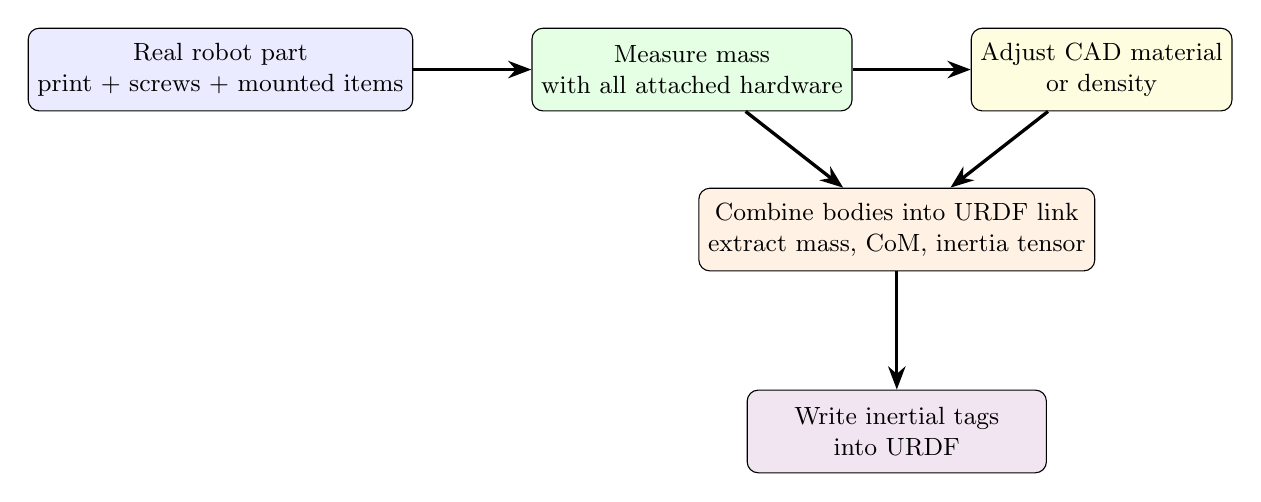
\begin{tikzpicture}[>=Stealth, node distance=1.6cm, every node/.style={font=\small, align=center}]
  \def\bw{3.15cm}
  \def\bh{1.05cm}

  \node[draw, rounded corners=4pt, fill=blue!8,
        minimum width=\bw, minimum height=\bh] (real)
        {Real robot part\\print + screws + mounted items};
  \node[draw, rounded corners=4pt, fill=green!10,
        minimum width=\bw, minimum height=\bh, right=1.5cm of real] (weigh)
        {Measure mass\\with all attached hardware};
  \node[draw, rounded corners=4pt, fill=yellow!12,
        minimum width=\bw, minimum height=\bh, right=1.5cm of weigh] (cadpart)
        {Adjust CAD material\\or density};

  \node[draw, rounded corners=4pt, fill=orange!10,
        minimum width=3.8cm, minimum height=\bh, below=1.5cm of $(weigh)!0.5!(cadpart)$] (combine)
        {Combine bodies into URDF link\\extract mass, CoM, inertia tensor};
  \node[draw, rounded corners=4pt, fill=violet!10,
        minimum width=3.8cm, minimum height=\bh, below=1.5cm of combine] (urdfout)
        {Write inertial tags\\into URDF};

  \draw[->, very thick] (real) -- (weigh);
  \draw[->, very thick] (weigh) -- (cadpart);
  \draw[->, very thick] (weigh) -- (combine);
  \draw[->, very thick] (cadpart) -- (combine);
  \draw[->, very thick] (combine) -- (urdfout);
\end{tikzpicture}
\caption{Hardware-to-CAD parameter flow.  The CAD model is used as an inertial bookkeeping tool after its mass properties are aligned with the real robot.}
\label{fig:hardware_to_cad_flow}
\end{figure}

\subsection{Rotor and Actuator Separation}

The transcript also highlights a more refined modeling step: separate the
actuator housing from the rotor where possible.  This is useful because the
rotor inertia may belong dynamically to a different side of the transmission
than the stator housing.  Even if the final URDF uses a simplified rigid-link
representation, thinking in terms of rotor-side and body-side inertia helps
avoid hiding major inertia in the wrong link.

\section{Actuator Model Calibration for Isaac Lab}

Once the URDF has credible rigid-body parameters, the next problem is actuator
fidelity.  A robot can still transfer poorly if the simulated actuator dynamics
do not match the real actuators.

The methodology in the transcript is straightforward:
\begin{enumerate}[leftmargin=2em]
  \item implement the same actuator-side behavior in simulation that is present on the real hardware,
  \item command the real actuator with simple test signals,
  \item run the same signals in simulation,
  \item compare encoder traces,
  \item tune actuator parameters until the responses are close.
\end{enumerate}

In the video, this includes adding acceleration-related behavior to the
simulated actuator model because the real actuator clearly behaves differently
with and without that effect.

\begin{figure}[H]
\centering
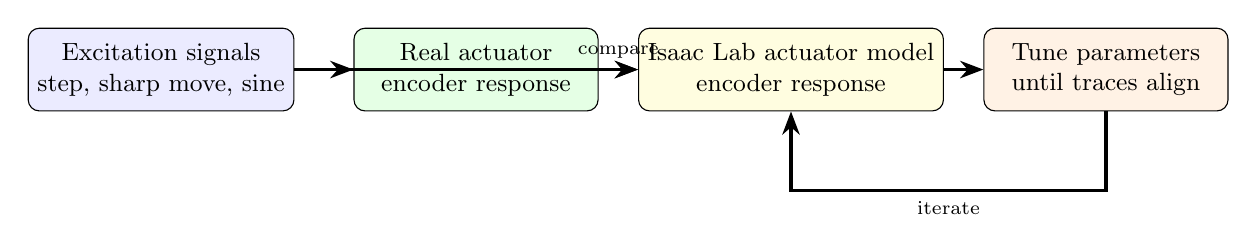
\begin{tikzpicture}[>=Stealth, every node/.style={font=\small, align=center}]
  \def\bw{3.1cm}
  \def\bh{1.05cm}

  \node[draw, rounded corners=4pt, fill=blue!8,
        minimum width=\bw, minimum height=\bh] (tests)
        at (0,0) {Excitation signals\\step, sharp move, sine};
  \node[draw, rounded corners=4pt, fill=green!10,
        minimum width=\bw, minimum height=\bh] (realact)
        at (4.0,0) {Real actuator\\encoder response};
  \node[draw, rounded corners=4pt, fill=yellow!12,
        minimum width=\bw, minimum height=\bh] (simact)
        at (8.0,0) {Isaac Lab actuator model\\encoder response};
  \node[draw, rounded corners=4pt, fill=orange!10,
        minimum width=\bw, minimum height=\bh] (tune)
        at (12.0,0) {Tune parameters\\until traces align};

  \draw[->, very thick] (tests) -- (realact);
  \draw[->, very thick] (tests) -- (simact);
  \draw[->, very thick] (realact) -- node[above,font=\scriptsize] {compare} (simact);
  \draw[->, very thick] (simact) -- (tune);
  \draw[->, very thick] (tune.south) -- ++(0,-1.0) -| node[pos=0.25, below,font=\scriptsize] {iterate} (simact.south);
\end{tikzpicture}
\caption{Actuator calibration loop: excite the real and simulated actuators with the same commands, compare encoder traces, and iterate on model parameters.}
\label{fig:actuator_calibration_loop}
\end{figure}

\subsection{Transcript-Based Identification Process: Sharp Command and Sine Wave}

The transcript describes a practical identification loop rather than a purely
analytical derivation.  The process is:
\begin{enumerate}[leftmargin=2em]
      \item choose one actuator at a time,
      \item command the real actuator with a \emph{sharp} move and with a
                        sinusoidal trajectory,
      \item apply the same commands to the simulated actuator model,
      \item log encoder response from both systems,
      \item tune the simulated actuator parameters until the traces are close.
\end{enumerate}

In the transcript, the important modeling decision was to add
\textbf{acceleration-related behavior} to the simulated actuator because the
real actuator clearly behaved differently with and without that effect.

\subsubsection{Step 1: Use a sharp command to identify transient behavior}

The transcript's ``sharp command'' is best interpreted as a fast setpoint
change or a high-jerk input used to expose transient effects.  This test is
useful for identifying:
\begin{itemize}[leftmargin=2em]
      \item command delay or dead time,
      \item rise time,
      \item acceleration limiting,
      \item overshoot,
      \item effective damping,
      \item saturation or clipping in the inner loop.
\end{itemize}

A useful low-order simulated position-actuator model is:
\begin{equation}
      \ddot q = \operatorname{sat}_{a_{\max}}\!\left(
      \omega_n^2\,(q_{\mathrm{cmd}} - q)
      - 2\zeta\omega_n\,\dot q
      \right),
      \label{eq:actuator_second_order_sat}
\end{equation}
where $\omega_n$ is the effective bandwidth, $\zeta$ is the damping ratio,
and $a_{\max}$ is an acceleration limit.

For a sharp command, the measured encoder trace is compared against the
simulated response to fit:
\begin{itemize}[leftmargin=2em]
      \item $a_{\max}$ from the initial slope and curvature,
      \item $\omega_n$ from how quickly the response rises,
      \item $\zeta$ from overshoot and settling behavior,
      \item explicit delay if the real actuator starts moving later than the model.
\end{itemize}

\subsubsection{Step 2: Use a sine wave to identify frequency response}

Once the transient response is roughly correct, the transcript's sinusoidal
test is used to check whether the actuator tracks periodic motion with the
correct amplitude and phase.

With a commanded signal
\begin{equation}
      q_{\mathrm{cmd}}(t) = A\sin(\omega t),
      \label{eq:sine_command}
\end{equation}
the measured actuator response can be approximated as
\begin{equation}
      q(t) \approx B(\omega)\sin\!\bigl(\omega t - \phi(\omega)\bigr),
      \label{eq:sine_response}
\end{equation}
where $B(\omega)$ is the output amplitude and $\phi(\omega)$ is the phase lag.

This test identifies:
\begin{itemize}[leftmargin=2em]
      \item actuator bandwidth,
      \item phase lag,
      \item high-frequency attenuation,
      \item lightly damped resonance or compliance effects.
\end{itemize}

In practice, one increases sine frequency gradually and checks whether the
simulated model loses amplitude and accumulates phase lag in the same way as
the real actuator.

\subsubsection{Step 3: Compare encoder traces and iterate}

The transcript's comparison variable is the encoder trace itself.  This is a
good practical choice because it avoids arguing about hidden internal states:
the only requirement is that the simulated actuator and the real actuator show
similar externally visible motion under the same test command.

The fitting loop is therefore:
\begin{enumerate}[leftmargin=2em]
      \item run a sharp command on the real actuator and log encoder position,
      \item run the same command in simulation and log simulated position,
      \item adjust delay, acceleration limit, damping, and bandwidth,
      \item run a sine-wave command at one or more frequencies,
      \item adjust the model until amplitude and phase match acceptably,
      \item repeat actuator by actuator.
\end{enumerate}

\begin{warnbox}
This procedure identifies the \emph{effective closed-loop actuator behavior},
not necessarily the internal motor physics in detail.  For direct-drive joints
that may be sufficient.  For cable-driven or SEA joints, the fitted response
can include motor dynamics, transmission compliance, cable damping, and pulley
effects all together.
\end{warnbox}

\subsubsection{Step 4: Apply the same idea to our planar cable-driven arm}

For our own planar robot, the same transcript methodology should be applied
joint by joint:
\begin{itemize}[leftmargin=2em]
      \item \textbf{Shoulder (AK80-kv60):} use sharp commands and sine waves to fit
                        the effective direct-drive actuator response.
      \item \textbf{Elbow (AK60-kv80 with steel cables):} use the same tests, but
                        interpret the identified model as actuator-plus-transmission behavior,
                        because the measured encoder response is influenced by cable stretch,
                        damping, pulley geometry, and any SEA element in the drive path.
\end{itemize}

For the elbow, a simple transmission-side quantity is the cable extension
\begin{equation}
      \delta = r_p(\theta_m - q_2),
      \label{eq:elbow_delta_methodology}
\end{equation}
which can be used in a compliant drive model such as
\begin{equation}
      F = k_s\,\delta + b_c\,\dot{\delta},
      \qquad
      \tau_2 = r_p F.
      \label{eq:elbow_force_methodology}
\end{equation}
The sharp and sine tests on the elbow then calibrate not only the motor-side
bandwidth, but also the effective compliance seen at the joint.

\subsection{Why This Calibration Matters}

If the rigid-body model is good but the actuator is too ideal in simulation,
the learned policy will exploit actuator behavior that does not exist on the
real robot.  Conversely, if the actuator model is close but the URDF inertial
properties are poor, the policy will still see the wrong dynamics.  Both must
be addressed together.

\section{Deployment Constraints Beyond the Physics Model}

The transcript also makes an important point that is easy to underestimate:
sim-to-real transfer is not only a physics problem.  It is also an
observation, estimation, and timing problem.

\subsection{Observation Availability}

The policy may require quantities such as:
\begin{itemize}[leftmargin=2em]
  \item joint positions and velocities,
  \item commanded body velocities,
  \item projected gravity from the IMU,
  \item base angular velocity,
  \item base linear velocity,
  \item previous action.
\end{itemize}

In the transcript, base linear velocity becomes the main obstacle because it is
not directly available from simple sensors and normally requires a state
estimator.  The practical workaround described there is to use a SLAM camera to
obtain pose and velocity signals directly, avoiding a full estimator in the
first iteration.

\subsection{Timing and Compute Path}

Even with a good model and a trained policy, deployment can fail if the sensing
and actuation loop cannot meet the required update rate.  The transcript gives
an example of a 50~Hz policy loop, implying a full sensor-read, policy, and
motor-command cycle of less than 20~ms.

This turns transport and compute hardware into part of the methodology:
\begin{itemize}[leftmargin=2em]
  \item CAN transport latency matters,
  \item loop-time consistency matters, not just mean latency,
  \item embedded compute choice changes inference and I/O jitter.
\end{itemize}

\begin{figure}[H]
\centering
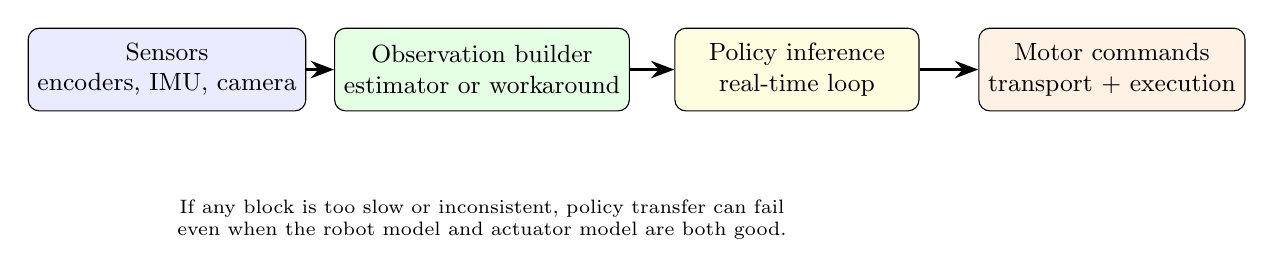
\begin{tikzpicture}[>=Stealth, every node/.style={font=\small, align=center}]
  \def\bw{3.1cm}
  \def\bh{1.05cm}

  \node[draw, rounded corners=4pt, fill=blue!8,
        minimum width=\bw, minimum height=\bh] (obs)
        at (0,0) {Sensors\\encoders, IMU, camera};
  \node[draw, rounded corners=4pt, fill=green!10,
        minimum width=\bw, minimum height=\bh] (state)
        at (4.0,0) {Observation builder\\estimator or workaround};
  \node[draw, rounded corners=4pt, fill=yellow!12,
        minimum width=\bw, minimum height=\bh] (policy)
        at (8.0,0) {Policy inference\\real-time loop};
  \node[draw, rounded corners=4pt, fill=orange!10,
        minimum width=\bw, minimum height=\bh] (motor)
        at (12.0,0) {Motor commands\\transport + execution};

  \draw[->, very thick] (obs) -- (state);
  \draw[->, very thick] (state) -- (policy);
  \draw[->, very thick] (policy) -- (motor);

  \node[font=\scriptsize, text width=10.5cm, below=1.0cm of state]
      {If any block is too slow or inconsistent, policy transfer can fail even when the robot model and actuator model are both good.};
\end{tikzpicture}
\caption{Deployment path for policy transfer.  Physics fidelity is necessary, but observation availability and timing consistency are also first-order constraints.}
\label{fig:deployment_path}
\end{figure}

\section{Methodology Adapted to Our Workflow}

For our own robotics workflow, the methodology can be written as:
\begin{enumerate}[leftmargin=2em]
  \item Measure each real rigid assembly carefully, including fasteners and attached components.
  \item Use CAD as an inertial bookkeeping tool, not just a geometry export tool.
  \item Populate URDF inertial tags from the corrected CAD model.
  \item Build or tune actuator dynamics in Isaac Lab or Isaac Sim using real actuator response data.
  \item Verify that the simulated actuator reproduces step and sinusoidal behavior seen on the real robot.
  \item Check whether the deployed policy's required observations are actually available on the hardware stack.
  \item Validate that the runtime platform can sustain the required control-loop period with acceptable jitter.
\end{enumerate}

\begin{resultbox}
The main methodological lesson is that sim-to-real success is not obtained by
``URDF only'' or ``policy only''.  It comes from three aligned layers:
accurate rigid-body parameters, calibrated actuator dynamics, and a hardware
runtime stack that can supply the required observations at the needed rate.
\end{resultbox}

\end{document}